\documentclass[conference,12pt]{IEEEtran}
\usepackage{filecontents}
\usepackage{cite}
\usepackage{color}
\usepackage{booktabs}
\usepackage[utf8]{inputenc}
\usepackage{color}
\usepackage{datetime}
\usepackage[pdftex]{graphicx}

%\usepackage[labelsep=space]{caption}
\DeclareGraphicsExtensions{.pdf,.jpeg,.png}
%\pagestyle{headings}

% correct bad hyphenation here
%\hyphenation{op-tical net-works semi-conduc-tor ATLAS FPGAs}

\begin{document}
% paper title
% can use linebreaks \\ within to get better formatting as desired
\twocolumn
\title{Simulating Weighted Decision Routing Based On Propagation Delay Using SuperSim
}

\author{\IEEEauthorblockN{Jonathan George}
\IEEEauthorblockA{
Colorado State University\\
Hewlett Packard Enterprise\\
jonathan.george@hpe.com
}
\and
\IEEEauthorblockN{Advised by: Nic McDonald}
\IEEEauthorblockA{
Hewlett Packard Enterprise\\
nicmcd@hpe.com
}
}
\vspace{3 in}
\maketitle


%\renewcommand*{\thefootnote}{\fnsymbol{footnote}}

\begin{abstract}
Choosing the proper path in complex interconnected networks, such as Dragonfly, has a significant impact on network latency. Adaptive Routing attempts to accomplish this, but there are many ways of implementing it. This paper attempts to improve on past work by accounting for propagation delay when selecting routes. Network experiments were run using SuperSim to test this idea. The result show that while there are some promising improvements, there needs to be additional work in this area before it is worth the cost of implementing this method.

\end{abstract}

%\IEEEpeerreviewmaketitle

\section{Introduction}
%Establish the topic
Creating the fastest and most powerful computers requires scale-able efficient interconnected networks are needed. The increasing rate of processor and memory innovation puts equal pressure to develop networks capable of creating powerful supercomputers by linking many of these powerful processors and memory banks together. 

%State your purpose
In searching for ways to improve these interconnected networks, routing algorithms stick out as a clear place to innovate. By creating adaptive routing which responds to congestion, we can achieve a significantly higher utilization of the router links thereby increasing bandwidth and decreasing cost.

Particularly the dragonfly topology requires adaptive routing because of the benefit of taking non-minimal paths during adversarial traffic patterns. Fat trees on the other hand always route minimally and see little benefit to adaptive routing. Due to it's high path diversity, a Dragonfly topology requires intelligent adaptive routing to be fully utilized cost efficiently.   
%Briefly summarize previous knowledge

%Establish Gap - 
Many of the previous adaptive algorithms suggested either require global congestion knowledge or can cause unnecessary latency if faced with an adverse traffic pattern. In many systems it is not feasible to have global congestion knowledge, therefore we need to address the latency problem. One particular issue which complicates things for adaptive routing is phantom congestion. Nic McDonald proposes that by accounting for the latency in the links, an adaptive routing algorithm could counteract phantom congestion and provide better bandwidth at full load and low latency under small loads. 

In this paper I explain adaptive routing as a concept, summarize previous work, discuss various interconnected networks, walk through the simulator setup and explore whether or not Nic's proposal of accounting for propagation delay is effective.


\section{Background}

In this section we will discuss the current state of adaptive routing algorithm in the context of the Dragonfly topology.

\subsection{Dragonfly Topology}

\begin{figure}[ht]
  \begin{center}
    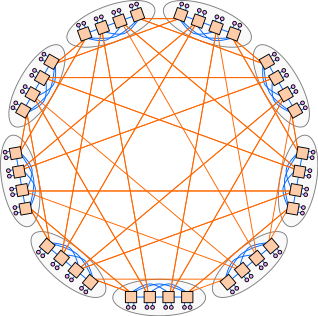
\includegraphics[width=2.5in,height=2.5in]{figures/Dragonfly-topology.png}
  \end{center}
   \vspace{-0.25in}
 \caption[Dragonfly Topology]{Dragonfly Topology}
 \label{fig:DragonFly}
\end{figure}

In this paper, I will be focusing on the Dragonfly topology.\cite{Dragonfly} Dragonfly is a  high-bandwidth topology proposed for large-scale networks in HPC systems. As shown in figure \ref{fig:DragonFly}, the topology uses a two tiers of routers consisting of a fully connected intra-group network (local) and a inter-group network (global). Each group uses a high-bandwidth, low latency local network which allows the group viewed as a virtual router. This allows abstraction when considering inter-group routing (figure \ref{fig:HyperX}). 

\begin{figure}[ht]
  \begin{center}
    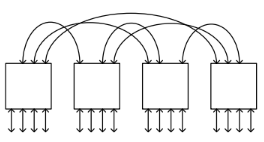
\includegraphics[width=3in,height=1.75in]{figures/HyperX.png}
  \end{center}
   \vspace{-0.25in}
 \caption{Abstracted view of Dragonfly's groups\cite{HyperX}}
 \label{fig:HyperX}
\end{figure}

Due to the large amount of path variety a packet could take to get to it's destination, Dragonfly requires adaptive routing to ensure balanced traffic patterns and good performance. 

\subsection{Adaptive Routing}
Traditional static routing always tries to take the minimal path to a packet's destination.  However, adaptive routing, in addition to the minimal path, bases it's output port decision on the state of the network. If the obvious shortest path is overly congested then it may be beneficial to take a longer route. 

Adaptive routing algorithms must be carefully tuned and balanced in order to ensure it takes the shortest route when traffic congestion is small and taking advantage of alternative routes when congestion is high. One such adaptive routing algorithm called Universal Globally-Adaptive Load-balanced routing (UGAL) was proposed by Arjun Singh.\cite{s05} The earliest form of this algorithm was a simple calculation to determine each path's cost (C) and always taking the lowest cost path. 

\[C = Q * H\]

UGAL calculates the current congestion of a path (Q) and multiplies it by the number of hops (H) to reach the destination. Calculating the exact congestion of a particular path is a non-trivial task. Look ahead congestion is too slow for adaptive routing and so Indirect Adaptive Routing (IAR) methods have been proposed over time to approximate it. This causes problems when the router's congestion doesn't match the entire path's congestion. In order to balance benign and adversarial traffic patterns, Jiang proposed adding a threshold (T) to the non-minimal paths.\cite{njd09} 

\[C_{nm} = Q_{nm} * H_{nm} + T\]

This threshold ensures that routers do not take non-minimal routes until there is sufficient congestion. This improves overall performance of the adaptive routing algorithm, but does not solve all of adaptive routing's problems. John Kim points out one such problem called phantom congestion.

\subsection{Phantom Congestion}

\begin{figure}[ht]
  \begin{center}
    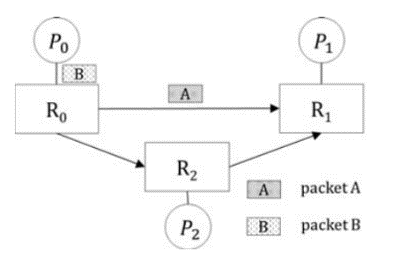
\includegraphics[width=3.0in,height=2.2in]{figures/PhantomCongestion.png}
  \end{center}
   \vspace{-0.25in}
 \caption[Dragonfly Topology]{3-node network example illustrating phantom congestion\cite{wkkjps15}}
 \label{fig:PhantomCongestion}
\end{figure}

Phantom congestion is the appearance of congestion when, in reality, there is none. John demonstrates this with a simple 3 router example. Assuming there is no other load in the network except two packets A and B and both packets are being sent sequentially from P0 to P1. While A is in flight, R0 will consider it as congestion because it is unsure of whether or not R1 will receive it. This can cause R0 to decide to potentially route B non-minimally even though there is no congestion at R1. The longer the latency between R0 and R1, the longer it will take R1 to acknowledge the receipt of A. This mean phantom congestion impacts longer paths more than short paths. This problem demonstrates the shortcoming of IAR and one of the main challenges to creating a good adaptive routing algorithm with limited information.


\section{Propagation Ratio}
%Discuss Nic's idea
Nic proposed that since phantom congestion is exasperated by longer paths, that we should try and prioritize taking shorter routes when we go non-minimal paths. His hope was that this would solve the phantom congestion problem and hopefully even remove the need for a threshold. This new variable we decided to call propagation ratio.

During my simulation I went through a few iterations of how to calculate the propagation ratio. Initially I just used the next hop's wire distance and divided by the wire width of the network. This was simplistic, but proved to cause non-minimal routes to be taken too often. I improved it by summing the next hop's wire distance plus the next hop's minimal route's wire distance before dividing by the wire width of the network. This causes routes which move closer to the destination, minimal and non-minimal, to have the same propagation ratio while longer wire distance paths are discouraged. By avoiding overshooting or backtracking, then we should be able to decrease the packet latency.

\[{PR} = \frac{L_{to\_next\_hop} + L_{next\_hop\_minimal}}{{Network Width}}\]

PR was applied to the equation by adding it to the congestion (Q). Instead of a threshold to the entire equation, SuperSim uses a congestion bias (b). This serves the same purpose of giving minimal routes priority in lower load situations. My equations became the following:

%(Q+PR+bias) * H
\[C_m = (Q + PR) * H\]

\[C_{nm} = (Q_{nm} + PR + b) * H_{nm}\]

%(Q+PR*W+bias) * H
To help tune my experiments I included a weighting (W). It was applied in the following way. 

\[C_m = (Q + PR * W) * H\]

\[C_{nm} = (Q_{nm} + PR * W + b) * H_{nm}\]

I also tried not applying the PR to the minimal case, but it had a little impact on the overall performance so I won't discuss the differences in this paper. There may be more to look at in this area, but my initial experiments were insufficient.

\section{Experiment}

Now that we have the proposed equation, we can discuss the simulator and it's configuration.

\subsection{SuperSim}
For this project, I used the SuperSim simulator created by Nic McDonald and others at HPE labs.\cite{SuperSim} SuperSim is an open source network simulator which is specifically designed for large-scale HPC networks. It is intended to help direct architecture design decisions and help promote both industry and academic research. 

%Why did I use it?
The primary reason why I used SuperSim was because I had easy access to the creator, Nic McDonald, but there are also several features which make SuperSim ideal for these kinds of experiments. First, SuperSim is very flexible and it was quite easy to make the adjustments to the routing algorithm and configure it while only rerunning the impacted simulations. Second, SuperSim is built on top of an effective task manager which takes full advantage of a computer's resources. This allowed me to complete my simulations quickly and iterate several times over the course of this project. 

SuperSim's sweep mode allows for in depth comparison of several variables. I was able to sweep over several values of my propagation ratio weight and different traffic patterns. My graphs were generated with sweeping each parameter with various loads at a 2\% step. Finally, SuperSim's built in graphing and graph viewing tools are effective at allowing for quick comparisons of the different simulations. 

%Topology setup
\subsection{Topology setup}
%Traffic patterns
As discussed earlier, I used the Dragonfly topology for my experiments. The number of groups (global width) was 33 and each group had 8 routers (local width). This gives a total of 264 routers in this network. SuperSim has already been used for simulating the dragonfly topology with varied wire latencies which is why I chose it over other similar topologies like HyperX. Future work could repeat this experiment on other topologies.

\subsection{Traffic Patterns}
For my experiments I used, two different traffic patterns to compare the impact of my algorithm, Uniform Random and Group Attack. 

%Uniform Random
Uniform Random (UR) demonstrates a fully load balanced scenario where each router is talking evenly to every other router. This traffic pattern is best handled by each router using the minimal route since every extra hop displaces another packet from entering the network. Adaptive Routing frequently struggles with performing well with this traffic pattern because the best choice is to always take minimal paths regardless of congestion.

%Worst Case Group Attack
Group Attack (GA) demonstrates a worst case scenario where one group is talking to only one other group. This concentrated traffic causes minimal routing to perform very poorly (about 10\% bandwidth on a Dragonfly) and requires taking non-minimal routes to achieve decent performance. 

The goal of any adaptive algorithm is to minimize any impact to UR patterns and get better performance from GA traffic patterns. This is how I will evaluate my results in the next section.


\section{Results}

In examining the results, it is most useful to first look at how often a minimal hop is taken verse a non-minimal hop in a GA simulation. Figure \ref{fig:loadavehops0} and \ref{fig:loadavehops25} show this for my baseline adaptive routing algorithm (weight=0) and when propagation ratio is applied (weight=0.25) respectively.

%WC Average hops graphs for primary impact on routes.
\begin{figure}[ht]
  \begin{center}
    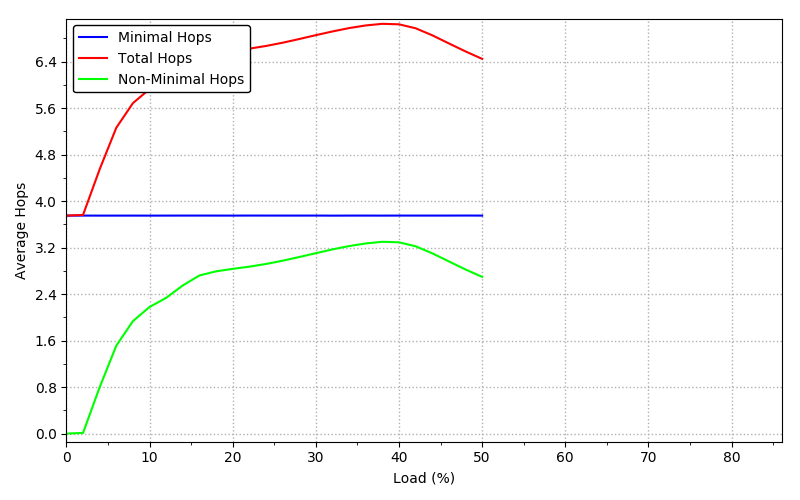
\includegraphics[width=3.4in,height=2.2in]{figures/loadavehops_GA_0.png}
  \end{center}
   \vspace{-0.25in}
 \caption[load average hops - 0 weight]{Average hops w/ WC traffic and PR weight=0}
 \label{fig:loadavehops0}
\end{figure}
\begin{figure}[ht]
  \begin{center}
    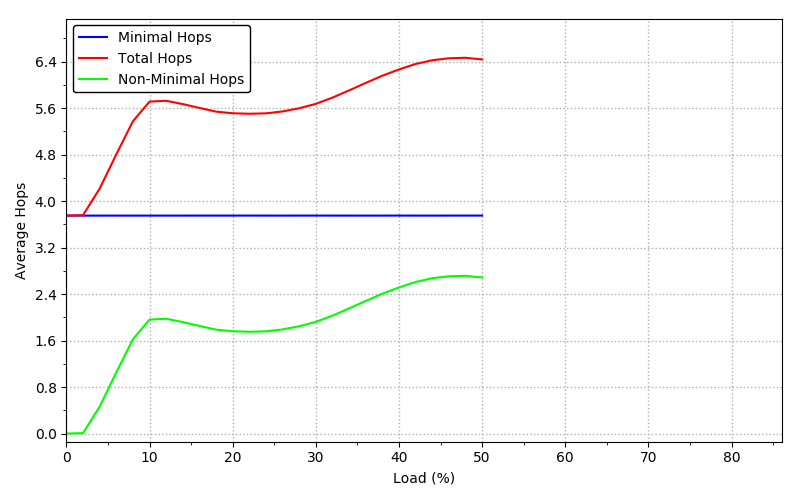
\includegraphics[width=3.4in,height=2.2in]{figures/loadavehops_GA_0_25.png}
  \end{center}
   \vspace{-0.25in}
 \caption[load average hops - 0.25 weight]{Average hops w/ WC traffic and PR weight=0.25}
 \label{fig:loadavehops25}
\end{figure}

Overall it can be seen that using propagation ratio does improve the adaptive routing algorithm by reducing the number of times a non-minimal route is used between 10\% and 45\%. Once congestion overcomes the congestion bias threshold at 10\%, my changes positively impact the number of hops, by leaning towards paths which bring the packet closer to the destination. Both graphs end at 50\% load at 6.4 average hops. Figure \ref{fig:loadlatcompGA} compares the mean latency between various weight values.

%WC Load latency compare graphs

\begin{figure}[ht]
  \begin{center}
    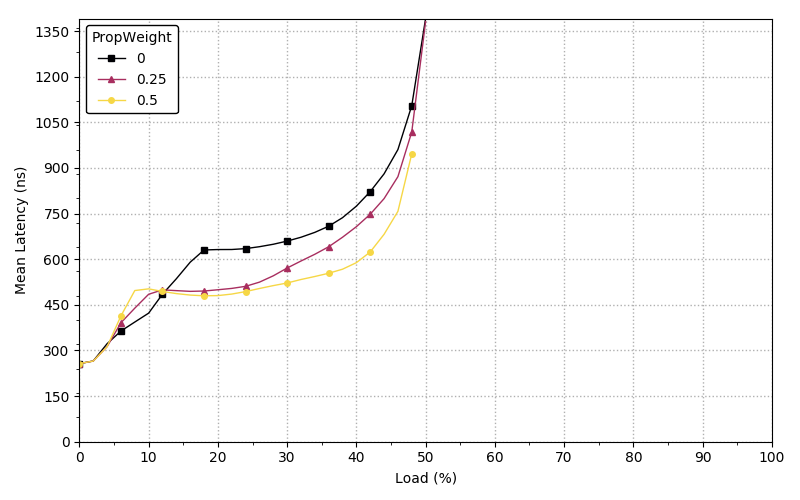
\includegraphics[width=3.4in,height=2.2in]{figures/loadlatcomp_GA_Mean.png}
  \end{center}
   \vspace{-0.25in}
 \caption[load latency compare GA mean]{Load vs mean latency weight comparison on WC}
 \label{fig:loadlatcompGA}
\end{figure}

Figure \ref{fig:loadlatcompGA} clearly matches the previous figures showing that the decrease in average hops results in a decreased latency. However, one interesting thing is that with a weight of 0.5, we never reach 50\% load instead our last point ends at 48\%. This indicates that at the propagation ratio causes us to approach an earlier asymptote. Likely 0.25 is reaching a slightly earlier asymptote as well, but my graphs do not have enough granularity (2\% step) to see it. This problem is seen more clearly while examining the uniform random load latency graph in figure \ref{fig:loadlatcompURmean}.


%UR impact
\begin{figure}[ht]
  \begin{center}
    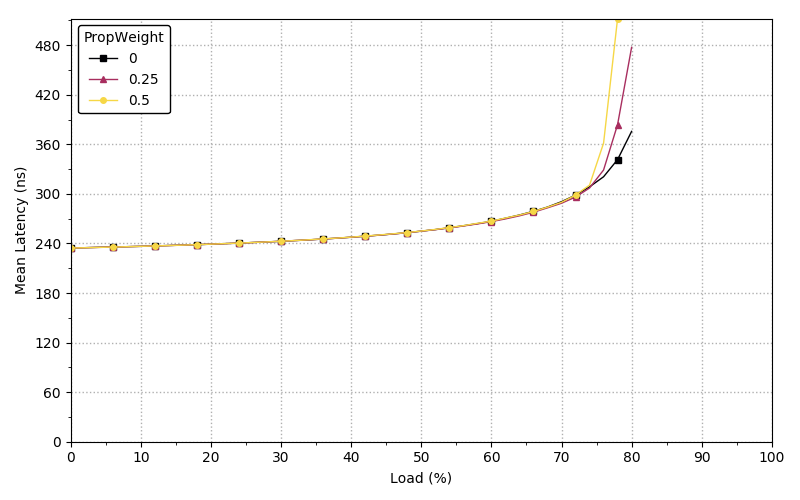
\includegraphics[width=3.4in,height=2.2in]{figures/loadlatcomp_UR_Mean.png}
  \end{center}
   \vspace{-0.25in}
 \caption[load latency compare UR mean]{Load vs mean latency weight comparison on UR}
 \label{fig:loadlatcompURmean}
\end{figure}

Figure \ref{fig:loadlatcompURmean} shows that unfortunately we will begin taking non-minimal paths slightly faster when using the propagation ratio. This cost to maximum load can erase any benefits to intermediate latency. This needs to be balanced depending on the application. 

\begin{figure}[ht]
  \begin{center}
    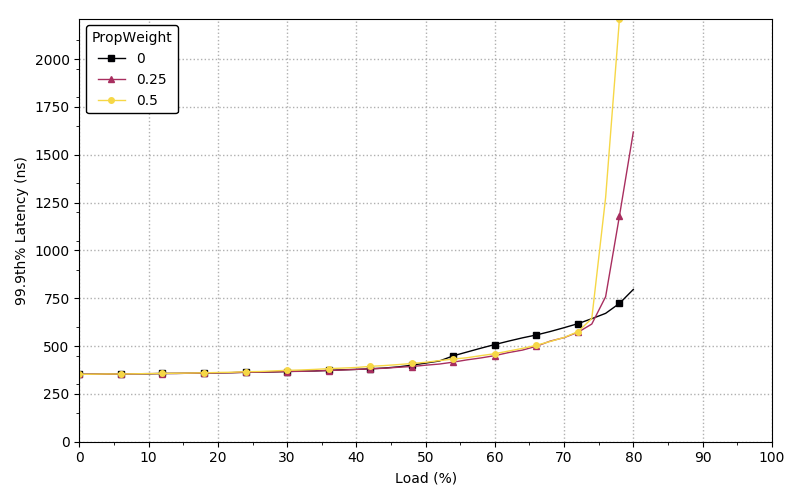
\includegraphics[width=3.4in,height=2.2in]{figures/loadlatcomp_UR_99_9.png}
  \end{center}
   \vspace{-0.25in}
 \caption[load latency compare UR 99.9\%]{Load vs 99.9\% latency weight comparison on UR}
 \label{fig:loadlatcompUR99}
\end{figure}

Figure \ref{fig:loadlatcompUR99} shows one last interesting find in the results. When looking at only the top 0.1\% highest latency values, then it is clear that propagation ratio is helping even the UR case from 50\% to 70\%. I think this is likely similar to increasing the threshold value. However, I haven't compared those two setting directly in this experiment.

\section{Conclusion}
%Explain why these shortcomings make this method not worth the trade offs. 

While propagation ratio has some interesting benefits, it seems like it unfortunately doesn't make the cut due to decreasing the maximum achievable bandwidth in both WC and UR traffic patterns. It is possible that this current equation would be beneficial if latency is more important than maximizing load.

This work could be continued and perhaps a better method of incorporating propagation ratio into adaptive router could be discovered. One potential idea would be to sweep over different biases and PR weights. It may be able to tune this algorithm further to make the downsides negligible while retaining the decreased mid-range latency. Additionally, further research into why propagation ratio negatively affects higher loads could help find ways to mitigate this issue.

\newpage
\bibliographystyle{IEEEtran}
\bibliography{IEEEabrv,references}




\newpage



\end{document}


